%! Author = Kevin Lin
%! Date = 11/12/2026

% Preamble
\documentclass[11pt,a4paper,margin=1in]{article}

% Packages
\usepackage{amsmath}
\usepackage{amssymb}
\usepackage{enumerate}
\usepackage{pdfpages}

\title{HW 7}
\author{Kevin Lin}
\date{11/12/2026}

% Document
\begin{document}
\maketitle

\section{}
Let $G \sim \mathcal{N}(0,I_n)$ and let $\Sigma^{1/2}$ denote the symmetric positive 
semidefinite square root of $\Sigma$. Then $X \overset{d}{=} \Sigma^{1/2}G$. Define
\begin{align*}
    g(z) &= f(\Sigma^{1/2}z) \\
    \nabla g(z) &= \Sigma^{1/2}\nabla f(\Sigma^{1/2}z), \\
    \|\nabla g(z)\|_2^2 &= \nabla f(\Sigma^{1/2}z)^\top \Sigma \nabla f(\Sigma^{1/2}z) \\
    &= \left\langle \Sigma\nabla f(\Sigma^{1/2}z),\nabla f(\Sigma^{1/2}z)\right\rangle
\end{align*}

Applying the Gaussian Poincare inequality to $g(G)$ gives
\begin{align*}
    \operatorname{Var}[f(X)]
    &= \operatorname{Var}[g(G)] \\
    &\leq E\|\nabla g(G)\|_2^2 \\
    &= E\left[\left\langle \Sigma\nabla f(X),\nabla f(X)\right\rangle\right]
\end{align*}
This proves the first inequality. For the second inequality, apply the Gaussian 
log-Sobolev inequality from $g$:
\begin{align*}
    \operatorname{Ent}(f(X)^2)
    &= \operatorname{Ent}(g(G)^2) \\
    &\leq 2E\|\nabla g(G)\|_2^2 \\
    &= 2E\left[\left\langle \Sigma\nabla f(X),\nabla f(X)\right\rangle\right]
\end{align*}
Thus, $\operatorname{Var}[f(X)] \leq E\left[\langle \Sigma\nabla f(X),\nabla f(X)\rangle\right]$
and $\operatorname{Ent}(f(X)^2) \leq 2E\left[\langle \Sigma\nabla f(X),\nabla f(X)\rangle\right]$.

\section{}
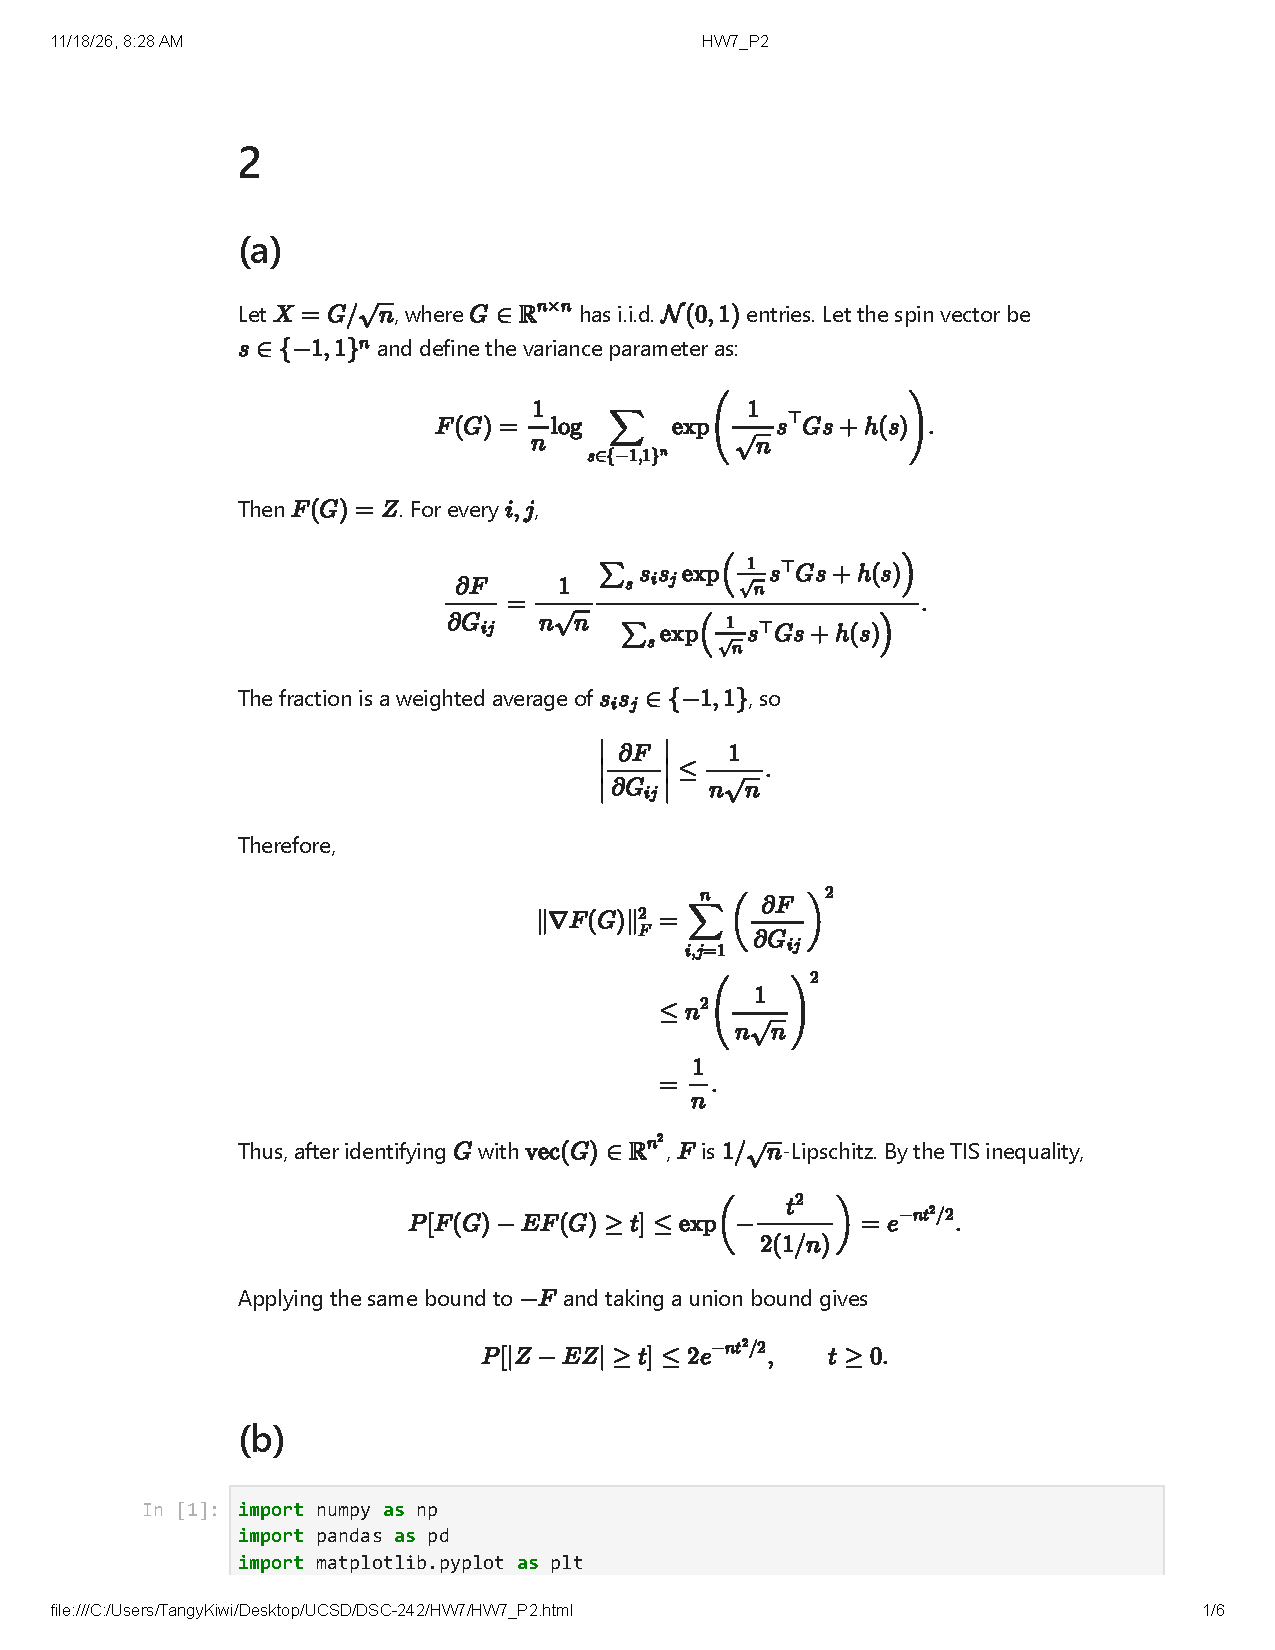
\includepdf[pages=-]{HW7_P2.pdf}

\section{}
\begin{enumerate}[(a)]
    \item Write expectations with respect to $p$ and $q$ as $E_p$ and $E_q$. For 
    $y\geq0$ and $t>0$, define
    \[
        \phi_t(y)=y\log y-y\log t-y+t
    \]
    From the hint,
    \[
        \operatorname{Ent}_q(Y)=\inf_{t>0}E_q[\phi_t(Y)]
    \]
    Also,
    \[
        \phi_t(y)=t\left[\frac{y}{t}\log\left(\frac{y}{t}\right)-\frac{y}{t}+1\right]\geq0
    \]
    because $u\log u-u+1\geq0$ for all $u\geq0$. Since $q/p\leq\omega$,
    \[
        E_q[\phi_t(f^2)] =\int \phi_t(f(x)^2)\frac{q(x)}{p(x)}p(x)\,dx \leq \omega E_p[\phi_t(f^2)]
    \]
    Taking the infimum over $t>0$ gives
    \[
        \operatorname{Ent}_q(f^2)\leq\omega\operatorname{Ent}_p(f^2)
    \]
    Since $p$ satisfies the log-Sobolev inequality,
    \[
        \operatorname{Ent}_p(f^2)\leq C_{\mathrm{LSI}}E_p[(f')^2]
    \]
    The lower density-ratio bound $q/p\geq\epsilon$ implies $p/q\leq1/\epsilon$, so
    \begin{align*}
        E_p[(f')^2] &= \int (f'(x))^2\frac{p(x)}{q(x)}q(x)\,dx \\
        &\leq \frac{1}{\epsilon}E_q[(f')^2]
    \end{align*}
    Combining the three inequalities,
    \[
        \operatorname{Ent}_q(f^2) \leq \frac{\omega}{\epsilon}C_{\mathrm{LSI}}E_q[(f')^2]
    \]
    Therefore, $q$ satisfies a log-Sobolev inequality with constant $\frac{\omega}{\epsilon}C_{\mathrm{LSI}}$.

    \item Let
    \[
        p(x)=\frac{e^{-x^2/2}}{\int_{\mathbb R}e^{-s^2/2}\,ds}
    \]
    be the standard Gaussian density. By the Gaussian log-Sobolev inequality, $p$ has $C_{\mathrm{LSI}}=2$.
    Write
    \[
        q(x)=\frac{e^{-V(x)}}{\int_{\mathbb R}e^{-V(s)}\,ds}
    \]
    Then
    \[
        \frac{q(x)}{p(x)}
        = C\exp\left(\frac{x^2}{2}-V(x)\right)
    \]
    for a positive constant $C$ independent of $x$. The assumption
    \[
        \frac{x^2}{2}+a\leq V(x)\leq \frac{x^2}{2}+b
    \]
    implies
    \[
        -b\leq \frac{x^2}{2}-V(x)\leq-a
    \]
    Therefore,
    \[
        Ce^{-b}\leq\frac{q(x)}{p(x)}\leq Ce^{-a}
    \]
    Taking $\epsilon=Ce^{-b}$ and $\omega=Ce^{-a}$ gives
    \[
        \frac{\omega}{\epsilon}=e^{b-a}
    \]
    Applying part (a) with $C_{\mathrm{LSI}}=2$ yields
    \[
        \operatorname{Ent}_q(f^2) \leq 2e^{b-a}E_q[(f')^2]
    \]
    Thus, for $X\sim q$,
    \[
        \operatorname{Ent}[f(X)^2]\leq2e^{b-a}E[f'(X)^2]
    \]
\end{enumerate}

\section{}
\begin{enumerate}[(a)]
    \item Fix $x,x'\in\mathbb R^n$. For any $y\in A_n$, the triangle inequality gives
    \[
        \|x-y\|_2\leq\|x-x'\|_2+\|x'-y\|_2
    \]
    Taking the minimum over $y\in A_n$ on the right-hand side,
    \[
        f_n(x)\leq\|x-x'\|_2+f_n(x')
    \]
    Hence,
    \[
        f_n(x)-f_n(x')\leq\|x-x'\|_2
    \]
    Interchanging $x$ and $x'$ gives
    \[
        f_n(x')-f_n(x)\leq\|x-x'\|_2
    \]
    Therefore,
    \[
        |f_n(x)-f_n(x')|\leq\|x-x'\|_2
    \]

    \item Suppose $x\in\{-1,1\}^n$ and $\sum_{i=1}^n x_i\geq\sqrt n$. For any 
    $y\in A_n$, $\sum_{i=1}^n y_i\leq0$, so
    \begin{align*}
        \sum_{i=1}^n(x_i-y_i) &=\sum_{i=1}^n x_i-\sum_{i=1}^n y_i \\
        &\geq\sqrt n.
    \end{align*}
    Since $x_i,y_i\in\{-1,1\}$, each $x_i-y_i\in\{-2,0,2\}$, and therefore
    \[
        x_i-y_i\leq(x_i-y_i)^2
    \]
    for every $i$. Summing gives
    \[
        \sqrt n\leq\sum_{i=1}^n(x_i-y_i)\leq\sum_{i=1}^n(x_i-y_i)^2
    \]
    Hence, for every $y\in A_n$,
    \[
        \|x-y\|_2^2\geq\sqrt n,
    \]
    so
    \[
        \|x-y\|_2\geq n^{1/4}.
    \]
    Taking the minimum over $y\in A_n$ gives
    \[
        f_n(x)\geq n^{1/4}
    \]

    \item Since $X\in\{-1,1\}^n$, $f_n(X)=0$ exactly when $X\in A_n$, or equivalently 
    when $\sum_iX_i\leq0$. The distribution of $\sum_iX_i$ is symmetric around zero, so
    \[
        P[f_n(X)=0] = P\left[\sum_{i=1}^nX_i\leq0\right]\geq\frac12
    \]
    By part (b),
    \[
        P[f_n(X)\geq n^{1/4}] \geq P\left[\sum_{i=1}^nX_i\geq\sqrt n\right]
    \]
    By the central limit theorem,
    \[
        \frac{1}{\sqrt n}\sum_{i=1}^nX_i\xrightarrow{d}\mathcal N(0,1)
    \]
    Since $1$ is a continuity point of the standard normal distribution,
    \[
        P\left[\sum_{i=1}^nX_i\geq\sqrt n\right]
        \longrightarrow P[G\geq1]=1-\Phi(1)>0,
    \]
    where $G\sim\mathcal N(0,1)$. Therefore,
    \[
        \liminf_{n\to\infty}P[f_n(X)\geq n^{1/4}]>0
    \]

    Let $Y=f_n(X)$ and let $Y'$ be an independent copy of $Y$. Recall that
    \[
        \operatorname{Var}(Y)=\frac12E[(Y-Y')^2]
    \]
    For all sufficiently large $n$, there is an absolute $c_0>0$ such that
    \[
        P[Y=0]\geq\frac12, \qquad P[Y\geq n^{1/4}]\geq c_0
    \]
    On the events $\{Y=0,Y'\geq n^{1/4}\}$ and $\{Y' =0,Y\geq n^{1/4}\}$, we have 
    $(Y-Y')^2\geq\sqrt n$. Thus,
    \begin{align*}
        \operatorname{Var}(Y) &=\frac12E[(Y-Y')^2] \\
        &\geq \frac12\sqrt n\left(P[Y=0]P[Y'\geq n^{1/4}]+P[Y'=0]P[Y\geq n^{1/4}]\right) \\
        &= \sqrt n\,P[Y=0]P[Y\geq n^{1/4}] \\
        &\geq \frac{c_0}{2}\sqrt n
    \end{align*}
    Therefore, $\operatorname{Var}(f_n(X))\geq c\sqrt n$ for an absolute constant 
    $c>0$ and all sufficiently large $n$.

    If $f_n(X)-Ef_n(X)$ were $\sigma^2$-sub-Gaussian with a variance proxy $\sigma^2$ 
    independent of $n$, then its log-MGF would satisfy
    \[
        \log E[e^{\lambda(f_n(X)-Ef_n(X))}]\leq\frac{\sigma^2\lambda^2}{2}
    \]
    Comparing second derivatives at $\lambda=0$ gives
    \[
        \operatorname{Var}(f_n(X))\leq\sigma^2,
    \]
    contradicting $\operatorname{Var}(f_n(X))\geq c\sqrt n\to\infty$. Hence no 
    $\sigma^2$ independent of $n$ can make $f_n(X)-Ef_n(X)$ sub-Gaussian.

    \item For $x\in\{-1,1\}^n$, let $x^{(i)}$ denote $x$ with coordinate $i$ flipped. 
    By convexity of $g$,
    \[
        g(x^{(i)})\geq g(x)+\langle\nabla g(x),x^{(i)}-x\rangle
    \]
    Since $x^{(i)}-x=-2x_ie_i$,
    \begin{align*}
        D_i g(x) &= g(x)-g(x^{(i)}) \\
        &\leq 2x_i\partial_i g(x).
    \end{align*}
    Therefore,
    \[
        (D_i g(x))_+\leq2|\partial_i g(x)|
    \]
    Summing the squares,
    \begin{align*}
        \sum_{i=1}^n(D_i g(x))_+^2 &\leq4\sum_{i=1}^n(\partial_i g(x))^2 \\
        &=4\|\nabla g(x)\|_2^2
    \end{align*}
    Since $g$ is differentiable and $1$-Lipschitz, $\|\nabla g(x)\|_2\leq1$. Thus,
    \[
        \sum_{i=1}^n(D_i g(x))_+^2\leq4
    \]
    Applying Theorem 15.2 with variance parameter $4$ gives
    \[
        P[g(X)-Eg(X)\geq t]\leq e^{-t^2/4}, \qquad t\geq0.
    \]

    \item Choose $x\in\{-1,1\}^n$ with the smallest possible positive coordinate sum:
    \[
        \sum_{i=1}^n x_i=
        \begin{cases}
            1, & n\text{ odd},\\
            2, & n\text{ even}
        \end{cases}
    \]
    Then $x\notin A_n$, but flipping any coordinate with $x_i=1$ produces a vector 
    in $A_n$. Any two distinct vertices of the hypercube are at Euclidean distance 
    at least $2$, while one such flip is at distance exactly $2$, so
    \[
        f_n(x)=2
    \]
    For every $i$ such that $x_i=1$, $x^{(i)}\in A_n$, so
    \[
        f_n(x^{(i)})=0,
        \qquad
        D_i f_n(x)=f_n(x)-f_n(x^{(i)})=2
    \]
    If $n$ is odd, the number of positive coordinates is $(n+1)/2$, and if $n$ is 
    even, it is $n/2+1$. Therefore,
    \[
        \sum_{i=1}^n(D_i f_n(x))_+^2
        \geq
        \begin{cases}
            4\frac{n+1}{2}=2n+2, & n\text{ odd},\\
            4\left(\frac n2+1\right)=2n+4, & n\text{ even}
        \end{cases}
    \]
    In either case,
    \[
        \sum_{i=1}^n(D_i f_n(x))_+^2\geq2n
    \]
    Thus the uniform discrete-gradient bound used in part (d) cannot hold with an 
    absolute constant for $f_n$.
\end{enumerate}

\noindent
\textbf{AI Usage:} All homework problems were written in VSCode and compiled using LaTeX
(Problem 2 utilized Jupyter notebook), with assistance from ChatGPT and Github
Copilot inline suggestions.

\end{document}
